\documentclass[crop,tikz]{standalone}%
\usetikzlibrary{calc}
\usepackage{amsmath, amsfonts}
\usetikzlibrary{calc, positioning, shapes.callouts}
\usepackage{filecontents}

\begin{document}
\begin{tikzpicture}
\def\abcsize{\normalsize}
\def\panelH{55 mm}
\def\panelW{165 mm}
\tikzstyle{panelstyle} = [draw=white, fill=white, rectangle, align = left, inner sep=0pt, minimum width= \panelW, minimum height = \panelH]
\node [panelstyle] (panel){};
\coordinate (corner) at (panel.north west);

\node (rt) at (corner) [anchor=north west, inner xsep=0pt, inner ysep=0pt, rectangle, minimum width= 27.5 mm, minimum height = \panelH, color=white, fill=white] {run and tumble};

\node (eps) at (corner) [anchor=north west, inner xsep=0pt, inner ysep=0pt] {

\includegraphics[trim={3mm 2mm 3mm 3mm}, clip, scale=0.73]{figures_eps/traj.eps}};
\node[anchor=west, black, black, thick] (targtext) at ($(corner) + (8mm, -10mm)$) {target};
\node[anchor=north, black!70!gray, text width=2cm, thin] (targtext) at (targtext.south) {\footnotesize(releasing\\ chemoattractant)};

\node[anchor=west, green!60!black] (runtext) at ($(corner) + (0mm, -34mm)$) {run};
\node[] (run) at ($(runtext) + (8mm, 0mm)$) {};
\draw[thin,->] (runtext) -- (run.center) node[anchor=center] {};

\node[anchor=east, blue] (tumbletext) at ($(corner) + (27.5mm, -22.5mm)$) {tumble};
\node[] (tumble1) at ($(corner) + (11mm, -25.5mm)$) {};
\draw[thin,->] (tumbletext) -- (tumble1.center) node[anchor=center] {};
\coordinate (corner) at (panel.south west);
\node[] (p) at ($(corner) + (10mm, 15mm)$) {};
\node[] (q) at ($(corner) + (17mm, 6mm)$) {};
\draw [<->, thick, black] (p.east) to[out=-20,in=100] (q);
\node[] (D) at ($(corner) + (19mm, 13mm)$) {$D_\mathrm{rot}$};
\node[teal!70!black] (D) at ($(corner) + (20mm, 3mm)$) {agent};

% run and tumble
%\node (rt) at (corner) [anchor=south west, inner xsep=0pt, inner ysep=0pt] {
%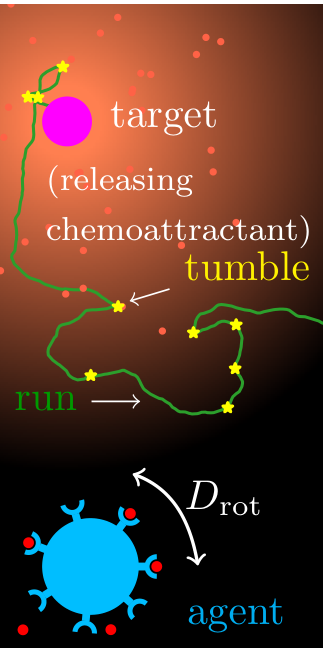
\includegraphics[trim={0 0 0 0}, clip, scale=1]{fig/figure0.eps}};
\node at (rt.north west) [anchor= north west, inner xsep=0pt, inner ysep=1pt] {\abcsize \textbf{(a)}};
\coordinate (corner) at (rt.south east);
\node (traj) at (corner) [anchor=south west, inner xsep=0pt, inner ysep=0pt] {
\includegraphics[trim={0 0 0 0}, clip, scale=0.98]{fig/trajectory_training.eps}};
\node at (traj.north west) [anchor= north west, inner xsep=0pt, inner ysep=1pt] {\abcsize \textbf{(b)}};
\coordinate (corner) at (traj.south east);
\node (weight) at (corner) [anchor=south west, inner xsep=0pt, inner ysep=0pt] {
\includegraphics[trim={0 0 0 0}, clip, scale=0.98]{fig/signal_weight.eps}};
%
\node at (weight.north west) [anchor= north west, inner xsep=0pt, inner ysep=1pt]{\abcsize \textbf{(c)}};
\node at (weight.south west) [anchor= south west, inner xsep=-3pt, inner ysep=20mm] {\abcsize \textbf{(d)}};
\coordinate (corner) at (weight.south east);
\node (sim) at (corner) [anchor=south west, inner xsep=0pt, inner ysep=0pt] {
\includegraphics[trim={0 0 0 0}, clip, scale=0.98]{fig/trajectory_simulation.eps}};
\node at (sim.north west) [anchor= north west, inner xsep=0pt, inner ysep=0pt] {\abcsize \textbf{(e)}};
\end{tikzpicture}
\end{document}


% latex  nvar_diagram.tex
% dvips figure.dvi -o figure.eps

